\subsection{VGGNet}
\begin{frame}{}
    \LARGE CNN Architectures: \textbf{VGGNet}
\end{frame}

\begin{frame}{VGGNet}
    \begin{itemize}
        \item \textbf{Improvement over AlexNet:} Uses a deeper network with small filters instead of a shallow network with larger filters.
        \item A stack of 3x3 conv layers (vs. 11x11 conv) has the same receptive field, more non-linearities, fewer parameters and deeper network representation.
        \item Two variants: VGG16 (13 conv + 3 FC layers) and VGG19 (16 conv + 3 FC layers).
    \end{itemize}

    \begin{figure}
        \centering
        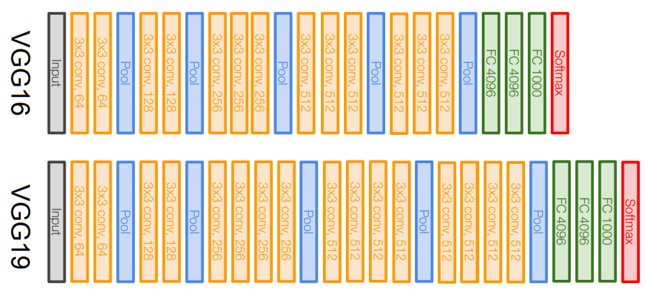
\includegraphics[width=1.0\textwidth,height=0.47\textheight,keepaspectratio]{images/cnn/VGG_16_19.png}
        \caption*{\scriptsize Figure: Stanford CS231n, Lecture~9; configurations D and E of Simonyan \& Zisserman, 2014 (Table~1).}
    \end{figure}
\end{frame}